% Theoretical background
%\clearpage % Uncomment if needed to force a page break before the chapter
\vspace{21.5pt}
\chapter{Teoreettinen tausta}

Jotta voidaan löytää pragmaattinen näkökulma funktionaaliseen ohjelmointiin, on käsiteltävä funktionaalisen ohjelmoinnin teoreettisia perusteita ja keskeisiä käsitteitä.

Tarkastellaan joukko-opin sovelluksia ohjelmoinnissa käytännön tasolla. Sivutaan kategoriateorian osuutta funktionaalisessa ohjelmoinnissa ilman syvällistä paneutumista yksityiskohtiin. Sivutaan myös \glsdisp{category_theory}{kategoriateoriaa}, joka on funktionaalisen ohjelmoinnin teoreettisen taustan kulmakivi. Tarkemmin käydään läpi kategoriateorian \glsdisp{monad}{monadi}-rakennetta, ja sen toimintaa.

Tutkitaan, miten nämä käsitteet integroituvat moderniin ohjelmistokehitykseen, kuten TypeScriptin käyttöön.

On tärkeää huomata, että tämän insinöörityön tavoitteena ei ole tarjota kattavaa opasta kaikkeen funktionaaliseen ohjelmointiin, vaan keskittyä valittuihin aihealueisiin, jotka tukevat työn pääteemoja ja osoittavat, miten teoreettiset käsitteet voidaan soveltaa käytännön ohjelmointihaasteisiin.

Valitut aihealueet pyritään avaamaan \glsdisp{language_agnostic}{kieliagnostisesti}, mutta kuitenkin JavaScript- sekä TypeScript-ekosysteemien näkökulmasta.

Lopulta näillä tiedoilla voidaan näyttää, miten funktionaalisen ohjelmoinnin käytänteet näkyvät hyödyllisesti (tai haitallisesti) ei-funktionaalisissa ohjelmistoprojekteissa.

Teoriaosuudessa pyritään pitämään sisältö mielenkiintoisena liimaamalla käsitteet yhdeksi kokonaisuudeksi. Teoriaan pyritään tuomaan konkretiaa erilaisilla esimerkeillä ja anekdooteilla.

\section{Funktionaalinen ohjelmointi}

Funktionaalinen ohjelmointi on ohjelmointiparadigma, jonka juuret ulottuvat 1930-luvulle ja lambda-kalkyylin kehitykseen. Lähestymistapa korostaa funktioiden käyttöä perusyksikköinä ja pyrkii välttämään \glsdisp{immutable_data}{muuttuvia tiloja} (mutability) sekä \glsdisp{side_effects}{sivuvaikutuksia} (side-effects). Funktionaalisen ohjelmoinnin keskeisiä käsitteitä ovat \glsdisp{pure_function}{puhtaat funktiot}, \glsdisp{higher_order_function}{korkeamman asteen funktiot}, \glsdisp{composed_function}{yhdistetyt funktiot}, sekä \gls{declarative_programming}. Funktiot ovat funktionaalisessa ohjelmoinnissa tosiaankin keskiössä. \citep{Tan2004,computerphile_lambda}

\subsection{Työn nimeämiskäytänteet}

Ohjelmoidessa funktionaalista ohjelmakoodia nimeämiskäytänteet ovat yhtä vaikeita kuin aina ennenkin. Tässä insinöörityössä käytetään Haskell-ohjelmoijien keskuudessa näkyviä nimeämiskäytänteitä, joissa käytetään lyhyitä ja \textquote{intuitiivisia} nimiä funktioille ja muuttujille. Esimerkiksi:

\begin{itemize}
    \item x: Yleisesti käytetty muuttuja tai parametri, joka edustaa arvoa, jota funktiot käsittelevät. Jos näkyvyysalalla on muita muuttujia, niitä nimetään usein aakkosjärjestyksessä x:stä eteenpäin (x, y, z).
    \item xs: Muuttuja, joka edustaa useita arvoja. Usein sisältää listan arvoista, mutta tietorakenteen tietäminen ei ole merkittävää.
    \item f: Yksittäinen funktio, jota voidaan käyttää käsittelemään arvoja. Jos näkyvyysalalla on muita funktioita, niitä nimetään usein aakkosjärjestyksessä f:stä eteenpäin (f, g, h, i...).
    \item fs: Muuttuja, joka edustaa useita funktioita. Usein sisältää listan funktioista, mutta tietorakenteen tietäminen ei ole merkittävää.
\end{itemize}

Esimerkkejä käytänteiden käytöstä:

\begin{code}
    \begin{minted}{javascript}
const map    = f => xs => xs.map(f)
const either = f => g => x => f(x) || g(x)
const max    = x => y => x > y ? x : y
const pipe   = fs => x => fs.reduce((acc, f) => f(acc), x)
\end{minted}
    \caption{Esimerkkejä insinöörityössä käytettävistä nimeämiskäytänteistä. Muunmuassa funktio \texttt{map} ottaa ensin yhden funktion (f), ja tämän jälkeen monta arvoa (xs). \texttt{Pipe} ottaa ensin monta funktiota (fs), ja tämän jälkeen yhden arvon (x)}
    \label{code:javascript_naming_convention_example}
\end{code}

\subsection{Puhtaat funktiot}

Funktionaalisessa ohjelmoinnissa \glsdisp{pure_function}{puhtaat funktiot} ovat funktioita, jotka poikkeuksetta aina palauttavat samalle syötteelle saman arvon. Funktion puhtauden voi päätellä siitä, jos sen voisi teoreettisesti korvata hakutaulukolla. \citep{feldman_fp_pragmatists}

Puhtaista funktioista hyötyy siten, että niitä voi käyttää uudelleen ja uudelleen kontekstista riippumatta. Puhtailla funktioilla voi rakentaa järjestelmäriippumattomia kirjastoja.

Puhtaiden funktioiden perusta on matematiikassa. Jos matemaattinen funktio $f(x) = x+2$ esimerkiksi ei aina palauttaisi samalle $x$ arvolle samaa palautusarvoa, mitä hyötyä funktiosta edes olisi? Toivottavasti $2 + 2$ tulee aina olemaan $4$.

\subsection{Kombinaattorit}

Funktionaalinen ohjelmointi mahdollistaa koodin uudelleenkäytettävyyden. Lambda-kalkyylin perustein joka ikisien ongelman voi purkaa pieniksi funktioiksi \cite{BlellochHarper2015}. Lambda-kalkyylistä johdetut kombinaattorit voi ottaa osaksi ohjelmoijan työkalupakkia missä tahansa ohjelmointikielessä, joka kohtelee funktioita samalla tavalla kuin muuttujia (first-class citizen) (Koodiesimerkki \ref{code:javascript_combinators}).

Jos kombinaattoreille haluaa etsiä vastaavanlaista määritelmää olio-ohjelmoinnin termeistä, voisi niitä ajatella olevan perustavanlaatuisia suunittelumalleja.

Kombinaattori \mintinline{javascript}|compose| on tapa tehdä yhdistettyjä funktioita, joista kerrotaan enemmän seuraavassa osassa.

\begin{code}
    \begin{minted}{javascript}
const identity      = x => x
const constant      = x => y => x
const apply         = f => x => f (x)
const thrush        = x => f => f (x)
const duplication   = f => x => f (x) (x)
const flip          = f => y => x => f (x) (y)
const compose       = f => g => x => f (g (x)) 
const substitution  = f => g => x => f (x) (g (x))
\end{minted}
    \caption{Yleiset kombinaattorit esitettynä JavaScriptissä \cite{javascript_combinators}. Kombinaattoreilla voi esittää lambda-kalkyyliä. Kombinaattoreilla voi muokata funktioiden toimintaa, ja yhdistää funktioita yhdiste funktioiksi}
    \label{code:javascript_combinators}
\end{code}

Kombinaattorit näyttävät uhkaavilta, ja raa'assa muodossaan niiden hyötyarvoa voi olla hankala havaita. Niiden käyttämistä voi kuitenkin perustella niiden perustavanlaatuisten ja kieliagnostisien ominaisuuksien takia. Ohjelmoidessa funktionaalisesti ei kombinaattoreita kuitenkaan tarvitse paljoa ajatella. Niitä tulee kirjoittamaan varmasti vähintään vahingossa, sillä niitä vaaditaan funktioita pyörittäessä \cite{javascript_combinators}. Kuitenkin on hyvä tiedostaa käytössä olevat rakennuspalikat, ja millä nimellä etsiä niistä tietoa tarvittaessa.

\subsection{Yhdistetyt funktiot ja niiden vahva merkitys}

Usein funktionaalista ohjelmointia mainostaessa puhutaan funktioiden puhtauden ja datan muuttumattomuuden olevan paradigman oleellisinta. Kuitenkin samaan aikaan juuri datan muuttumattomuus ja tilattomuus koetaan paradigman suureksi kompastuskiveksi \cite{cantarella_fp_haitat,is_reduce_bad,vakil2016}.

On tärkeää huomata, että kaiken ei tarvitse olla täysin puhdasta ja muuttumatonta, kunhan ne osat, joissa funktionaalista ohjelmointia hyödynnetään, pysyvät ennustettavina ja hallittavina.

\glsdisp{composed_function}{Yhdistetyt funktiot} ovat loistava tapa kirjoittaa selkeää ja modulaarista koodia. Parasta on, että kaiken ei tarvitse olla pelkkiä funktioita: voi hyvin kirjoittaa myös olio-ohjelmointityylillä ja silti hyödyntää yhdistettyjä funktioita logiikan selkeyttämiseksi ja yksinkertaistamiseksi.

Loppujen lopuksi funktionaalisen ohjelmoinnin perusta on funktioissa ja niiden yhdistämisessä. Datan muuttumattomuus ja sivuvaikutuksettomuus on vain esivaatimus funktioiden ennustettavuudelle.

\glsdisp{composed_function}{Yhdistetty funktio} tarkoittaa yksinkertaisesti kahden, tai useamman, funktion yhdistämistä siten, että yhden funktion tulos syötetään seuraavalle. Esimerkiksi koodiesimerkin \ref{code:javascript_manual_composition} funktio $h$ on funktioiden $f$ ja $g$ yhdiste. Ajaessa funktio $h$, suoritetaan ensin $g$, jonka palautusarvo annetaan funktiolle $f$. Kaksi funktiota yhdistämällä on saatu yksi uusi funktio.

\begin{code}
    \begin{minted}{javascript}
const f = x => 2 * x

const g = x => x + 3

const h = x => f(g(x))
\end{minted}
    \caption{JavaScript-esimerkki yhdistetystä funktiosta h ilman pipe tai compose funktiota}
    \label{code:javascript_manual_composition}
\end{code}

Funktionaalisissa ohjelmointikielissä yhdistettyjä funktioita pystyy usein kirjoittamaan käyttäen kieleen sisäänrakennettuja operaattoreja, joilla funktioiden yhdistäminen on helppoa ja suoraan osana ohjelmointikieltä \cite{fsharpcomposition,haskellcomposition}.
JavaScriptissä ei ole vastaavanlaista sisäänrakennettua operaattoria.
(Vaikkakin sellainen on ollut kehitteillä \cite{tc39_pipeline_operator}.)
Operaattorin voi kuitenkin kirjoittaa funktiona helposti osaksi mitä tahansa koodikantaa (Koodiesimerkki \ref{code:javascript_pipe_composition}).

\begin{code}
    \begin{minted}{javascript}
const pipe    = f => g => x => g(f(x))
const compose = f => g => x => f(g(x))

const h = pipe(f)(g)
// tai vaihtoehtoisesti
const h = compose(g)(f)
\end{minted}
    \caption{JavaScript-esimerkki funktiokompositiosta pipe ja compose funktioilla}
    \label{code:javascript_pipe_composition}
\end{code}

Voi olla mielenkiinoista huomata, että koodiesimerkin \mintinline{javascript}{compose} löytyy myös koodiesimerkin \ref{code:javascript_combinators} tunnetuista yleisistä kombinaattoreista.

Koodiesimerkissä \ref{code:javascript_pipe_composition} on näytettynä kaksi eri tapaa yhdistää funktioita: \texttt{pipe} ja \texttt{compose}. Käytännössä tapojen ainoa ero on se, kummasta suunnasta funktiot suoritetaan. \texttt{compose} on lähempänä yhdistettyjen funktioiden matemaattisia perusteita, kun taas \texttt{pipe} on usein helpompi lukea, sillä se suoritetaan yleisessä lukemissuunnassa, eli vasemmalta oikealle, tai ylhäältä alas. \citep{whyprefercompose}

Tulevissa koodiesimerkeissä tullaan suosimaan funktioiden yhdistämistä käyttäen \texttt{pipe}-funktiota \texttt{compose}-funktion sijasta.

Esimerkin \ref{code:javascript_pipe_composition} \texttt{pipe} ja \texttt{compose} toimivat vain kahdelle funktiolle kerrallaan. Tämä tapa seuraa lambda-kalkyyliä \cite{computerphile_lambda}. Ohjelmointikielen mukaan voi kuitenkin olla mieluisaa kirjoittaa funktiot niin, että ne tukevat suoraan mielivaltaista määrää funktioita.

JavaScriptissä näin voi tehdä esimerkiksi hyödyntämällä Array-tietorakennetta (Koodiesimerkki \ref{code:javascript_better_pipe}).

\begin{code}
    \begin{minted}{javascript}
const pipe    = fs => x => fs.reduce((acc, f) => f(acc), x)
const compose = fs => x => fs.reduceRight((acc, f) => f(acc), x)

const f = x => x + 1
const g = x => x * 2
const h = x => x - 3

const i = pipe([f, g, h])
i(5) // (((5 + 1) * 2) - 3) = 9
// tai vaihtoehtoisesti
const i = compose([h, g, f])
i(5) // (((5 + 1) * 2) - 3) = 9
\end{minted}
    \caption{JavaScript-esimerkki yhdistettyjen funktioiden luomisesta käyttäen \texttt{reduce} ja \texttt{reduceRight} funktioita. Nämä versiot voivat ottaa mielivaltaisen määrän funktioita argumenttina}
    \label{code:javascript_better_pipe}
\end{code}

Mikä tästä sitten tekee loistavaa? Se, että ohjelmointi on kerrankin oikeasti kuin LEGO palikoilla leikkimistä (Koodiesimerkki \ref{code:javascript_composition_example}).

\begin{code}
    \begin{minted}{javascript}
const pipe     = fs => x => fs.reduce((acc, func) => func(acc), x)
const multiply = x => y => x * y
const add      = x => y => x + y
const filter   = f => xs => xs.filter(f)
const map      = f => xs => xs.map(f)
const isEven   = x => x % 2 === 0

const rejectOdds   = filter(isEven)
const multiplyBy10 = multiply(10)

const pipeline = pipe([rejectOdds, map(multiplyBy10)])

pipeline([1, 2, 3, 4]) // [20, 40]
\end{minted}
    \caption{JavaScript-esimerkki yhdistettyjen funktioiden käyttämisestä laskutoimituksiin. Erilaiset operaatiot on pilkottu uudelleenkäytettäviksi funktioiksi}
    \label{code:javascript_composition_example}
\end{code}

Esimerkissä näytetyt funktiot ovat hyvin yksinkertaisia. Kuitenkin ne ovat täysin uudelleenkäytettäviä. Jos totuttautuu käyttämään joitain funktioita kaikissa projekteissa, voi huomata koodin kirjoittamisen tehokkuuden ja johdonmukaisuuden kasvavan.

\section{Tyyppiteoria ja joukko-oppi}
Tämä osa pyrkii kirjoittamaan matemaattisista käsitteistä käytännönläheisesti ja mahdollisesti suuresti yksinkertaistaen. Ajatuksena on, että ylemmän tason ajattelumalli välittyisi tekstissä tarkkojen määritelmien sijasta.

Joukko-oppi on matematiikan haara, joka tutkii joukkojen ominaisuuksia ja niiden välisiä suhteita. Ohjelmoinnissa joukko-oppi ilmenee yksinkertaisimmin joukko-tietorakenteiden kautta, jotka mahdollistavat uniikkien alkioiden käsittelyn tehokkaasti ja ilmaisuvoimaisesti \cite{mdn_set,mdn_set_methods}. On myös luotu ohjelmointikieli, joka perustuu kokonaan joukko-oppiin \cite{SETL_SET_LANGUAGE}.

Tyyppiteoria puolestaan on matematiikan haara, joka tutkii arvojen luokittelua, ja miten niitä käsitellään ohjelmoinnissa ja logiikassa \cite{type_theory,algebraic_data_types}.

Tyyppien ja joukkojen semanttinen ero on nyanssinen \cite{type_vs_set}. Ohjelmoinnissa puhutaan usein tyypeistä. Insinööriopintojen matematiikassa joukot ovat olleet vahvasti läsnä. Tässä osassa pääajatuksena on miettiä, kuinka asiat muutetaan funktioilla toisiksi, asiat voi mieltää kuuluvan joukkoihin tai tyyppeihin, kumpaa nyt ymmärtää paremmin. Oikea määritelmä saattaa lähestyä \glsdisp{category_theory}{kategoriateoriaa}, mutta erottaminen ei liene olevan tällä tasolla relevanttia.

Ihmisillä on kuitenkin kyky hahmottaa asioita joukkoina (tai tyyppeinä). Koko maailman voi mallintaa niillä (Kuva \ref{fig:fruit_set}) \cite{algebraic_data_types}.

\begin{figure}[ht]
    \centering
    \AltText{Omena, päärynä ja banaani.}{
\includegraphics[width=10cm]{HEDELMIA}}
    \caption{Mihin joukkoon tai tyyppiin nämä saattaisivat kuulua \cite{viljofruits}?}
    \label{fig:fruit_set}
\end{figure}

Koska koko maailman voi mallintaa joukkoina (tai tyyppeinä), voidaan niillä mallintaa myös ohjelmia.


\subsection{Joukko-tietorakenne}

Ohjelmoinnissa joukko-tietorakennetta käytetään hyvin laajasti, ja sen merkitys on keskeinen monissa ohjelmointikielissä, kuten Pythonissa, Javassa ja JavaScriptissä. Joukko-tietorakenne mahdollistaa alkioiden tallentamisen ilman duplikaatteja. Sen operaatiot, kuten unioni, leikkaus ja erotus, ovat suoraan peräisin matemaattisesta joukko-opista. Joukko-tietorakenteen tehokkuus ja yksinkertaisuus tekevät siitä tehokkaan työkalun monenlaisissa sovelluksissa. \citep{mdn_set,ecma_spec}

Joukko-tietorakenne kuvaa joukko-opin joukkoa. Joukko-tietorakenteessa säilytetään kokoelma uniikkeja alkioita. Joukko-tietorakenne on ohjelmoinnissa mieluinen työkalu sen tehokkuuden ansiosta. \citep{ecma_spec}

Kokemusten mukaan ohjelmoija ei usein mieti joukko-tietorakennetta matemaattisista lähtökohdista. Tästä kuitenkin voisi olla hyötyä, sillä Joukko-opin periaatteiden ymmärtäminen ja soveltaminen ohjelmoinnissa ei ainoastaan tehostuskeino, vaan myös laajentaa näkemystä siitä, miten abstraktit matemaattiset konseptit voidaan muuttaa konkreettisiksi työkaluiksi. Tämä yhdistelmä tarjoaa ohjelmoijille sekä teoreettisen että käytännöllisen perustan, joka on arvokas monissa erilaisissa sovelluksissa ja ongelmanratkaisutilanteissa \cite{bartosz_category_for_progamers}.

\subsection{Funktioilla joukoista toisiin}
Kun ohjelmoinnissa pohditaan joukko-opin hyödyntämistä, kehittyy \glsdisp{language_agnostic}{kieliriippumaton} kyky kirjoittaa koodia. Kun miettii, mitä ylipäätään voi laskea, pääsee ohjelmoinnissa omalle abstraktille tasolle. \citep{Tan2004,BlellochHarper2015}

Matemaattisesti joukkojen välille voidaan tehdä kuvauksia, tai toisin sanoen funktioita. Merkintä funktiosta, joka \textquote{muuttaa} joukon $A$ joukoksi $B$, on esimerkiksi yksinkertaisesti $A \to B$ \cite{mellin2005joukkooppi}. Funktio muuttaa minkä tahansa joukon $A$ alkion joksikin joukon $B$ alkioksi.

Funktionaalisessa ohjelmoinnissa puhtaiden funktioiden voidaan ajatella aina olevan rinnastettaessa jonkin joukon muutokseksi johonkin toiseen joukkoon (Esimerkkikoodi \ref{code:ts_set_example}) \cite{bartosz_category_for_progamers}. (Toisaalta funktioiden argumentit ja palautusarvot ovat aina joukkoja riippumatta siitä onko funktio puhdas vai ei. Ei-puhtaat funktiot eivät kuitenkaan välttämättä luo yksikäsitteisiä muutoksia joukkojen alkioille.)

\begin{code}
    \begin{minted}{typescript}
type SetA = 'a' | 'b' | 'c'
type SetB = 1 | 2 | 3
const aToB = (a: SetA): SetB => {
    switch (a) {
        case 'a': return 1
        case 'b': return 2
        case 'c': return 3
    }
}  
\end{minted}
    \caption{Havainnollistava funktio, joka muuttaa joukon A, \{a,b,c\}, joukoksi B, \{1, 2, 3\}}
    \label{code:ts_set_example}
\end{code}

Tarkastellaan konkreettisempaa esimerkkiä lähtien koodiesimerkistä \ref{code:ts_set_theory_3}.

\begin{code}
    \begin{minted}{typescript}
const divide = (x:number) => (y:number) => x / y
\end{minted}
    \caption{Funktio, joka jakaa numeron toisella}
    \label{code:ts_set_theory_3}
\end{code}



Funktio ottaa kaksi numeroa, ja jakaa ensimmäisen toisella. Argumentit on tyypitetty JavaScript-numeroiksi. Jos kyseistä funktiota haluaa käyttää, ohjelmoijan tulisi tietää, että nollalla ei voi jakaa, ja että jos niin kuitenkin tehdään, JavaScript palauttaa arvon \mintinline{javascript}|Infinity| (tai erityisemmässä tapauksessa \mintinline{javascript}|NaN|) (Koodiesimerkki \ref{code:ts_division}).


\begin{code}
    \begin{minted}{typescript}
console.log(1/0)  // Infinity
console.log(1/-0) // -Infinity
console.log(0/0)  // NaN
\end{minted}
    \caption{Jakamisoperaattorin toiminta JavaScriptissä}
    \label{code:ts_division}
\end{code}

Jos jakolaskufunktion kehitykseen halutaan soveltaa joukko-oppia, voi olla mieluista määritellä argumenteille spesifimmät joukot, sillä joukkona JavaScriptin \mintinline{javascript}|number| sisältää epämieluisia arvoja laskujen kannalta (\mintinline{javascript}|[NaN, Infinity, -Infinity]|).

Voidaan luoda jakolaskua varten joukot \mintinline{javascript}|Rational| ja \mintinline{javascript}|NonZero|, ja ohjelmoida ne TypeScript tyypeiksi (Koodiesimerkki \ref{code:ts_type_mayhem}).

\begin{code}
    \begin{minted}{typescript}
const RationalSymbol = Symbol('Rational')
const NonZeroSymbol = Symbol('NonZero')

type Rational = number & { [RationalSymbol]: "brand" }
type NonZero = Rational & { [NonZeroSymbol]: "brand" }

const isRational = (x: number): x is Rational => 
    ![Infinity, -Infinity, NaN].includes(x)
const isNonZero = (x: number): x is NonZero => 
    isRational(x) && x !== 0
\end{minted}
    \caption{Rational ja NonZero joukkojen määritelmät TypeScriptissä}
    \label{code:ts_type_mayhem}
\end{code}

Ajatuksena on, että joukko \mintinline{javascript}|Rational| sisältää kaikki JavaScriptin tukemat rationaaliluvut, ja että joukko \mintinline{javascript}|NonZero| muuten sama paitsi ilman nollaa (Kuva \ref{fig:set-esimerkki}).



\begin{figure}[ht]
    \centering
    \AltText{Joukko NonZero on joukon Rational aito osajoukko. Joukko Rational on joukon number aito osajoukko.}{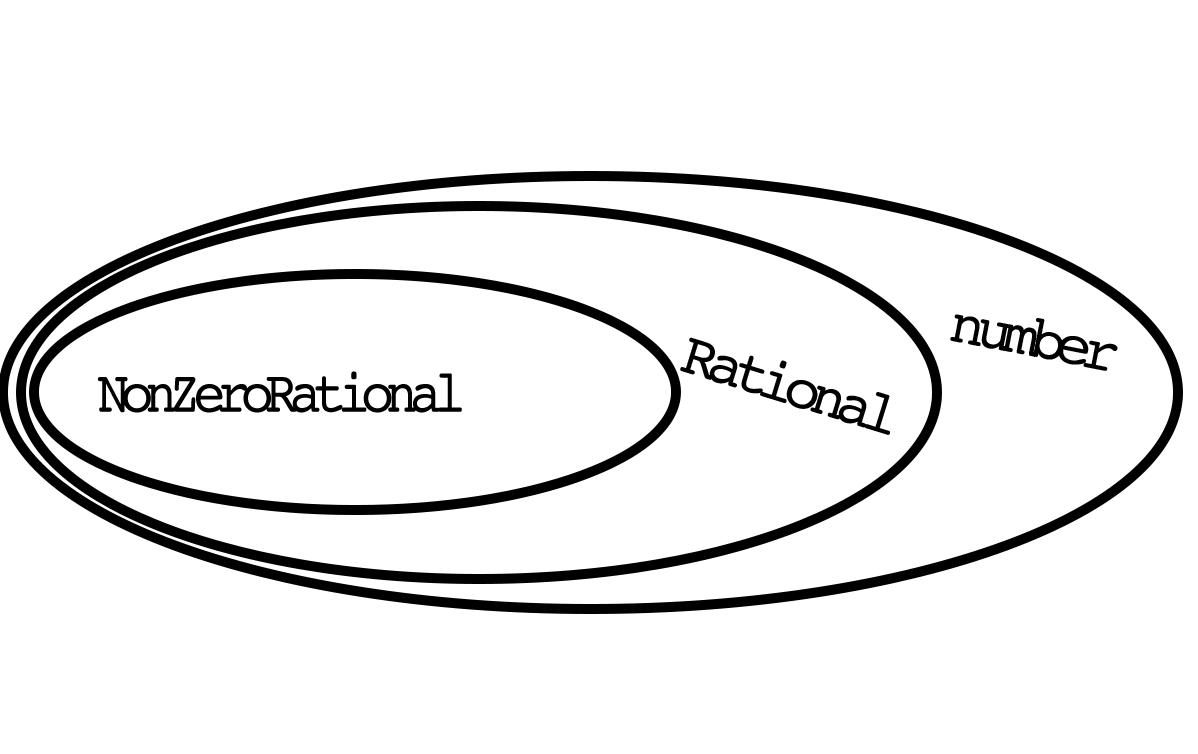
\includegraphics[width=7.1cm]{set_esimerkki}}
    \caption{Joukot NonZero, Rational ja number esitettynä osajoukkoina}
    \label{fig:set-esimerkki}
\end{figure}


Jos jakamisesimerkkiin määritetään joukot funktion argumenttien oikeiksi rajoitteiksi, ei funktiota voi käyttää väärin. TypeScript ei anna ajaa koodia, jos arvojen ei ole varmistettu kuuluvan oikeisiin joukkoihin (Koodiesimerkki \ref{code:ts_set_theory_6}) \cite{typsecript_website}.

\begin{code}
    \begin{minted}{typescript}
const divide = (x: Rational) => (y: NonZero) => x / y as Rational
\end{minted}
    \caption{Korrekti versio. Funktiolle annettavat arvot on varmistettava kuuluvan oikeisiin joukkoihin jossain vaiheessa ennen funktioon syöttöä käyttäen määriteltyjä \mintinline{javascript}|isRational| ja \mintinline{javascript}|isNonZero| funktioita }
    \label{code:ts_set_theory_6}
\end{code}

Aiempaan esimerkkiin voisi päätyä vaikkei olisi koskaan kuullut joukko-opista. Päällimmäisenä ajatuksena on kuitenkin se, että jos syötteitä ja palautusarvoja miettii joukkojen kannalta, syntyy luotettavampaa ohjelmakoodia ja vähemmän yllätyksiä. Tyypit ovat jo itsessään joukkoja, mutta niiden yksityiskohdat riippuvat käytössä olevasta, esimerkiksi ohjelmointikielen, tyyppijärjestelmästä \cite{type_theory}. Siksi ajatuksen tasolla joukkojen ajattelu on hyödyllistä.

Argumentit ja palautusarvot (tyypit) voi tietysti mieltää joukkoina myös \glsdisp{composed_function}{yhdistetyissä funktioissa} (Kuva \ref{fig:function_composition_in_sets}). Vaikka ohjelmoinnissa joukko-oppia ei rinnasteta ainoastaan funktionaaliseen ohjelmointiin,  joukko-opin ajattelu on siinä vähintäänkin tervetullutta.

\begin{figure}[htbp]
    \centering
    \begin{tikzpicture}
        % Ellipses for sets A, B, and C with background colors
        \draw[thick, ellipse, fill=green!20] (0,0.875) ellipse (0.8cm and 1.75cm);  % Set A with light blue background
        \draw[thick, ellipse, fill=blue!20] (3,0.875) ellipse (0.8cm and 1.75cm); % Set B with light green background
        \draw[thick, ellipse, fill=red!20] (6,0.875) ellipse (0.8cm and 1.75cm);   % Set C with light red background

        % Nodes for set A (without borders)
        \node[draw=none] (A1) at (0,2) {1};
        \node[draw=none] (A2) at (0,1.25) {2};
        \node[draw=none] (A3) at (0,0.5) {3};
        \node[draw=none] (A4) at (0,-0.25) {4};

        % Nodes for set B (without borders)
        \node[draw=none] (B1) at (3,2) {A};
        \node[draw=none] (B2) at (3,1.25) {B};
        \node[draw=none] (B3) at (3,0.5) {C};
        \node[draw=none] (B4) at (3,-0.25) {D};

        % Nodes for set C (without borders)
        \node[draw=none] (C1) at (6,2) {$\alpha$};
        \node[draw=none] (C2) at (6,1.25) {$\beta$};
        \node[draw=none] (C3) at (6,0.5) {$\gamma$};
        \node[draw=none] (C4) at (6,-0.25) {$\delta$};

        % Arrows from A to B
        \draw[->] (A1) -- (B1);
        \draw[->] (A2) -- (B3);
        \draw[->] (A3) -- (B2);
        \draw[->] (A4) -- (B4);

        % Arrows from B to C
        \draw[->] (B1) -- (C2);
        \draw[->] (B2) -- (C1);
        \draw[->] (B3) -- (C3);
        \draw[->] (B4) -- (C4);

        % Labels for sets
        \node[draw=none, text=green!50!black] at (-.5,3.25) {$A = \{1,2,3,4\}$};
        \node[draw=none, text=blue] at (3,3.25) {$B = \{A,B,C,D\}$};
        \node[draw=none, text=red] at (6.5,3.25) {$C = \{\alpha, \beta, \gamma, \delta\}$};

        % Arrow to new diagram
        \draw[->, line width=1.5mm, black] (3,-1.25) -- (3,-2.25) node[midway, right] {};

        % Corrected ellipses for sets A and C below the original picture
        \draw[thick, ellipse, fill=green!20] (0,-4.125) ellipse (0.8cm and 1.75cm);  % Set A with light blue background
        \draw[thick, ellipse, fill=red!20] (6,-4.125) ellipse (0.8cm and 1.75cm);   % Set C with light red background

        % Corrected nodes for set A (without borders) - Lower position
        \node[draw=none] (A1b) at (0,-3) {1};
        \node[draw=none] (A2b) at (0,-3.75) {2};
        \node[draw=none] (A3b) at (0,-4.5) {3};
        \node[draw=none] (A4b) at (0,-5.25) {4};

        % Corrected nodes for set C (without borders) - Lower position
        \node[draw=none] (C1b) at (6,-3) {$\alpha$};
        \node[draw=none] (C2b) at (6,-3.75) {$\beta$};
        \node[draw=none] (C3b) at (6,-4.5) {$\gamma$};
        \node[draw=none] (C4b) at (6,-5.25) {$\delta$};

        % Direct arrows from A to C (composition)
        \draw[->] (A1b) -- (C2b);
        \draw[->] (A2b) -- (C3b);
        \draw[->] (A3b) -- (C1b);
        \draw[->] (A4b) -- (C4b);
    \end{tikzpicture}
    \vspace{10pt}
    \caption{Funktioiden yhdistäminen joukko-opin näkökulmasta. Funktiot A$\,\to\,$B ja B$\,\to\,$C yhdistämällä saadaan A$\,\to\,$C. Älykkäällä kääntäjällä voi poistaa turhia laskutoimituksia. Keskimmäisen joukon evaluointi on käytännössä turhaa, jos funktiot ovat puhtaita}
    \label{fig:function_composition_in_sets}
\end{figure}


\subsection{Kategoriateoria}


Joukko-oppi ei ole ainoa ohjelmointiin sovellettava matemaattinen osa-alue. Funktionaaliselle ohjelmoinnille oleellisin ja syvällisin osa-alue on \gls{category_theory} \cite{bartosz_category_for_progamers,promises-spec-94,dear_functional_bros}.


Kategoriateoria tutkii matemaattisia rakenteita ja niiden välisiä suhteita erittäin abstraktilla tasolla. Se keskittyy objektien (kuten joukkojen tai tyyppien) ja niiden välillä olevien morfismien (funktioiden tai muunnosten) tutkimiseen \cite{bartosz_category_for_progamers}. Kategoriateorian avulla voidaan ymmärtää ja formalisoida monimutkaisia matemaattisia ja ohjelmallisia rakenteita. \cite{bartosz_category_for_progamers,promises-spec-94,category_theory}
Kategoriateoriaa ohjelmoijille opettavan Bartosz Milewskin kokemusten mukaan, vaikka algebra tai kalkyyli olisi ohjelmoijalle ajatuksena hirveää, kategoriateoria on kuitenkin erityisen mieluisaa sen suuresta teoreettisuudesta huolimatta. \cite[9]{milewski2017category}.

Kategoriateoriassa peruspalikat ovat kategoriat \cite[9]{milewski2017category}. Kategoria on rakenne, joka koostuu morfismeista. Esimerkiksi joukot ja funktiot koostavat kategorian, jossa joukot ovat kategorian objektit, ja funktiot kategorian morfismit \cite{category_theory}. Kategoriateoriaan ei perehdytä tarkemmin tässä työssä Monadi-rakennetta lukuun ottamatta. Ei ole käytännönläheistä tuoda tavattoman teoreettisia käsitteitä työhön, jossa tavoitteena on etsiä jonkin kaltaista konkretiaa.


\section{Monadi}

Monadi tulee esille funktionaalisessa ohjelmoinnissa erittäin usein. Se on alun perin teoreettinen rakenne, joka on löytynyt 1900-luvun puolivälin jälkeen kategoriateoriaa tutkivien matemaatikkojen ansiosta \cite{Beck2003}. Monadin hyöty ohjelmoinnissa ilmeni vasta myöhemmin 1990-luvulla \cite{computerphile_monad}.

Ohjelmoinnissa monadilla voidaan hallita sivuvaikutuksia, ketjuttaa operaatioita ja yhtenäistää abstraktioita \cite{computerphile_monad,bartosz_category_for_progamers_10,stackoverflow_what_monad}. Ohjelmoinnissa monadi on kieliagnostinen käsite.

Tässä osassa käydään läpi, mitä ovat yleiset monadit, miten implementoida monadi, miten niitä käytetään, ja lopulta pyritään tiivistämään miten monadeja voi ajatella ohjelmoinnissa.

\subsection{Yleiset monadit}

\texttt{Promise, Maybe, Either, Result, State, IO, ja Lista (Array)}. Nämä ovat esimerkkejä yleisesti käytetyistä monadeista. \cite{monad_wikipedia,bartosz_category_for_progamers_10}

Pintapuolisesti tarkasteltuna esitetyt käsitteet vaikuttavat hyvin erilaisilta, sillä niiden käyttötarkoitukset ja rakenteet vaihtelevat merkittävästi. Esimerkiksi \texttt{Promise} käsittelee asynkronisia operaatioita, kun taas \texttt{Maybe} kuvastaa mahdollisia arvoja, jotka voivat olla olemassa tai olla olematta. \texttt{Either} ja \texttt{Result} tarjoavat mekanismin virheiden käsittelyyn, ja \texttt{State} mahdollistaa tila-arvojen kantamisen funktioiden läpi. \texttt{IO} käsittelee sivuvaikutuksia, ja \texttt{Lista (Array)} tarjoaa toistuvien arvojen käsittelyn.

Kuitenkin näitä kaikkia yhdistää yhteinen abstraktio. Ne kaikki toteuttavat tietyt perustoiminnot \texttt{bind} (\texttt{flatMap/chain}) ja \texttt{of} (\texttt{unit/pure}). Näiden operaatioiden avulla monadit voivat kapseloida laskennan tilan tai sivuvaikutuksen, tarjoten yhdenmukaisen tavan yhdistää operaatioita ja siirtää tietoa laskentaketjujen läpi.

JavaScriptissä \mintinline{js}|Array| toteuttaa toiminnon \texttt{bind} \mintinline{js}|Array.prototype.flatMap|-metodilla, ja \texttt{of} toiminnon staattisella \mintinline{js}|Array.of|-metodilla \cite{stackoverflow_flatmap_monad,stackoverflow_js_array_monad}.


JavaScriptin \mintinline{js}|Promise| toteuttaa toiminnon \texttt{bind} \mintinline{javascript}|Promise.prototype.then|-metodilla, ja \texttt{of} toiminnon staattisella \mintinline{javascript}|Promise.resolve| ja \mintinline{javascript}|Promise.reject| metodeilla \cite{read-it-later-11481,stackoverflow:why_monad,promises-spec-94}.

Vaikka JavaScriptin \mintinline{js}|Promise| ja \mintinline{js}|Array| toteuttavatkin monadin \texttt{bind} ja \texttt{of} toiminnot, se ei tee niistä automaattisesti monadeja kategoriateorian tai funktionaalisen ohjelmoinnin sääntöjen mukaan \cite{promises-spec-94,stackoverflow:why_monad,stackoverflow_js_array_monad}. Kehittäjä Jake Archibaldin mukaan akateemisten käsitteiden seuraaminen puhtaasti ei kuitenkaan usein johda käytännölisiin ratkaisuihin \cite{pennane_fp_gist}. Tästä syystä on kohtuullista puhua näistä rakenteista monadeina, vaikkeivat ne sitä puhtaasti olisikaan.


\subsection{Monadin implementointi}

Konkreettisesti monadilla tulee siis olla kaksi toimintoa: \texttt{of} ja \texttt{bind}. Toiminto \texttt{of} käärii arvoja monadiin. Toiminnon voidaan ajatella olevan monadin konstruktori. \citep{stackoverflow_what_monad}

\texttt{Bind}-toiminnolla muutetaan monadiin käärittyä arvoa antamalla toiminnolle funktio, joka palauttaa toisen saman tyypin monadin. \cite{stackoverflow_what_monad} \texttt{Bind}-toiminto on käytännössä sama kuin tunnetumpi \texttt{map}-toiminto. Erona on, että \texttt{map} palauttaa muokatun arvon, joka on kääritty samaan monadiin, kun taas \texttt{bind} mahdollistaa monadin sisällä olevan arvon muuttamisen ja sen ketjuttamisen muihin monadisiin operaatioihin.

Näillä kahdella toiminnolla voidaan luoda rakenteita, jotka käyttäytyvät kuin monadi. Monadin täydet hyödyt eivät kuitenkaan ilmene, jos rakenne ei myös täytä monadien kolmea sääntöä: vasen identiteetti (left identity), oikea identiteetti (right identity), ja liitännäisyys (associativity) \cite{haskellmonadlaws}. Jos kaikki kolme sääntöä toteutuu, voidaan luoda työkaluja, joissa voidaan käyttää mitä tahansa monadia, ja silloin monadi on määritelmän mukaisesti monadi.

Osassa \textquote{Promise-tietorakenne on miltei monadi} puidaan sitä, miksei JavaScriptin \texttt{Promise} ole määritelmällisesti täydellisesti monadi, ja miksei ilman ulkoisia kirjastoja JavaScriptiin voida enää tuoda määritelmän täyttäviä monadeja. Kuitenkin rakenne, joka on kuin monadi, voi myös olla erittäin hyödyllinen. Siksi ei tarkemmin käsitellä, miten monadin määritelmän voi oikeellisesti täyttää.


\subsection{Monadin käyttäminen}

Monadeja käytetään operaatioiden ketjuttamiseen. Monadeilla voi käytännössä tehdä yhdistettyjä funktioita, joissa on mukautettu tapa hallita mitä yhdisteen funktiokutsujen välissä tapahtuu.

Käydään esimerkkinä JavaScriptin \texttt{Promise}-tietorakennetta (joka toimii kuin monadi) (Koodiesimerkki \ref{code:promise_monad_concise}).

\begin{code}
    \begin{minted}{typescript}
fetch("https://some.imaginary.api.com/v1") 
    .then(result => result.json()) 
    .then(data => data.users)
    .then(users => users.map(user => user.id))
    .catch(error => Array.of()) 
    \end{minted}
    \caption{Promise-tietorakenteella bind-operaatioden ketjutus, jossa haetaan käyttäjätietoja kuvitteellisesta ulkoisesta rajapinnasta. Jos mikään yksittäinen askel päätyy virhetilaan, palauttaa ohjelma tyhjän listan kutsumalla \mintinline{js}|Array.of|-metodia}
    \label{code:promise_monad_concise}
\end{code}

Koodiesimerkissä nähdään operaatioiden monadinen ketjutus. Jokainen \mintinline{js}|Promise.then|-kutsu palauttaa aina uuden Promise-monadin. Jos jokin yksittäinen Promise päätyy virhetilaan, ei enää seuraavia then-kutusja ajeta, vaan ketju päätyy automaattisesti \texttt{catch}-osioon.

Käytännössä koko ohjelma on siis vain yhdistetty funktio, jossa ollaan määritelty räätälöityä logiikkaa siihen, miten funktiokutsut käsitellään. Kuitenkaan \mintinline{js}|Promise.catch| ei liity suoraan monadisuuteen, eikä käytännössä oikeellisesti implementoidun monadin tarvitsisi käyttää sellaista \cite{promises-spec-94}.

Raja on häilyvä. Onko JavaScriptin Promise monadi vai ei? Matemaatikkojen mielestä monadi on \textquote{yksinkertaisesti} monoidi endofunktoreiden kategoriassa \cite{bartosz_category_for_progamers_10,monad_wikipedia,stackoverflow_what_monad}. Toisten mielestä monadi on asia, jolla on \texttt{flatMap}-metodi \cite{stackoverflow_flatmap_monad}.

Pragmaattisuuden nimissä monadi saa tässä työssä olla rakenne, jolla voidaan ketjuttaa operaatioita itsemäärittelemällä tavalla, joka mahdollisesti eroaa tavallisesta funktioiden yhdistämisestä.


\section{Pragmaattisuus funktionaalisessa ohjelmoinnissa}

Funktionaalisen ohjelmoinnin iskevin teoria on pitkälti käytynä, ja on ehkä selvää, että funktionaalinen ohjelmointi on pohjimmiltaan erittäin teoreettista. Voi pohtia, miten funktionaalinen ohjelmoinnin voi tuoda ohjelmistokehittäjän arsenaaliin käytännönläheisesti.

Kun funktionaalisen ohjelmoinnin kauneus on matemaattisissa kulmakivissä, joilla ei ole tapaa taipua, miten sen voi yhdistää säännöttömään JavaScriptiin, tai muuhun vastaavanlaiseen ohjelmointikieleen?

Mikä on se lähestymistapa, jota tarvitaan käytännönläheiseen, pragmaattiseen, funktionaaliseen ohjelmointiin?

Robert C. Martinin mukaan pragmaattinen funktionaalinen ohjelmointi on sitä, että käytetään esimerkiksi \glsdisp{immutable_data}{muuttumattomuutta} ja puhtaita funktioita silloin, kun ne parantavat ohjelman luettavuutta, ylläpidettävyyttä ja suorituskykyä, ja kuitenkin niin, ettei vaadita täydellistä sitoutumista funktionaalisen ohjelmoinnin paradigmaan. \citep{martin2017pragmaticfp}

Myös Cantarella mainitsee opinnäytetyönsä loppupuolella ajatuksen, että mitä enemmän paradigmoihin liittyviin artikkeleihin perehtyy, sitä myötämielisemmäksi tulee ajatukselle, että paradigmoja tulisi yhdistellä vapaammin. \citep[45]{cantarella_fp_haitat}

Myös kokemusten perusteella työpaikalla on havaittu funktionaalisen ohjelmoinnin toimivan kohtuullisen hyvin ripoteltuna proseduraalisen ohjelmakoodin.

Pragmaattista funktionaalista ohjelmointia vaikuttaa siis olevan se, että otetaan vain mitä tarvitaan \cite{dear_functional_bros,martin2017pragmaticfp,cantarella_fp_haitat}. Toisaalta se, mitä tarvitaan ei ole välittömästi selvää. Toisille pragmaattista on jättää kaikki matemaattinen teoria pois ohjelmoinnista heti kättelyssä, toisille kategoriateorian rakenteiden käyttäminen, kun ne oikeasti sopivat mallintamaan ongelmaa \cite{holvikari2021category,martin2017pragmaticfp}.

Tässä insinöörityössä tarkempia pragmaattisia funktionaalisen ohjelmoinnin käytäntöjä pyritään tuomaan esille neljännessä osassa \textquote{Funktionaalisia käytänteitä ei-funktionaalisissa ohjelmointikielissä}, ja siitä eteenpäin.

\section{Funktionaalinen ohjelmointi \& TypeScript}
JavaScript ei ole funktionaalinen ohjelmointikieli, vaikka se funktionaalisuutta tukeekin \cite{is_reduce_bad}. TypeScriptin tyyppijärjestelmällä funktionaalisesta ohjelmoinnista saa jo mieluisampaa \cite{holvikari2021category}.

JavaScriptia halutaan käyttää kaikkeen ohjelmointiin, vaikka usein erinäköisiin tehtäviin olisi parempiakin ohjelmointikieliä tarjolla. Voi itse päättää, onko pragmaattista käyttää kaikkeen samaa työkalua, ja säästää opiskelussa, vai käyttää aikaa uuden sopivamman työkalun löytämiseen, ja säästää toteuttamisessa.


\subsection{Kielen sopivuus funktionaaliseen ohjelmointiin}

Vaikka TypeScript ei ole pohjimmiltaan funktionaalinen ohjelmointikieli, on sillä ominaisuuksia, joilla funktionaalisesta ohjelmoinnista tulee verraten helppoa.

TypeScriptissä on käytännössä kolme eri tapaa määrittää funktioita (Esimerkkikoodi \ref{code:javascript_function_types}). Nuolifunktioilla voidaan harjoittaa funktionaaliselle ohjelmoinnille tyypillistä argumenttien yksi kerrallaan antamista.


\begin{code}
    \begin{minted}{typescript}
function rnd(min: number, max: number) { 
	return Math.floor(Math.random() * max) + min;
}
const rnd2 = (min, max) => Math.floor(Math.random() * max) + min;
const rnd3 = min => max => Math.floor(Math.random() * max) + min;
\end{minted}
    \caption{Kolme eri tapaa kirjoittaa funktio JavaScriptissä \cite{okhravi-g-discussion}. Funktiomäärittely, funktioilmaus ja osittain sovellettava funktioilmaus}
    \label{code:javascript_function_types}
\end{code}

Koska funktioita voi käyttää JavaScriptissä kuin muuttujia (first-class citizen), voi niitä antaa argumentteina toisille funktioille (Koodiesimerkki \ref{code:js_first_class}). Tämä mahdollistaa funktionaaliselle ohjelmoinnille tyypillisten \glsdisp{higher_order_function}{korkeamman asteen funktioiden} luomisen, ja käyttämisen.

\begin{code}
    \begin{minted}{javascript}
function A()  { return "moi"; }
function B(f) { return f(); }
B(A) // "moi"
\end{minted}
    \caption{Funktioiden ensiluokkaisuus JavaScriptissä. Funktiolle B voidaan antaa funktio argumenttina}
    \label{code:js_first_class}
\end{code}

Funktionaalisen ohjelmoinnin piireissä TypeScriptin tyyppijärjestelmää arvostetaan myös, koska sillä voidaan rakentaa algebrallisia datatyyppejä, jotka ovat yleisesti puhtaissa funktionaalisissa ohjelmointikielissä läsnä ja suuressa roolissa \cite{holvikari2021category}.


\subsection{Algebralliset datatyypit}

TypeScriptin tyypit ovat mieluisia funktionaaliselle ohjelmoinnille. TypeScript mahdollistaa funktionaaliselle ohjelmoinnille olennaisten algebrallisten datatyyppien määrittelemistä \cite{holvikari2021category}.

Algebralliset datatyypit ovat osa funktionaalisen ohjelmoinnin maailmaa. Niiden käyttämisen on huomattu olevan järkevää ja luontevaa \cite{holvikari2021category,hickey_maybe_not,algebraic_data_types}

Yksinkertaisesti algebralliset datatyypit ovat keino määritellä ja käsitellä monimutkaisia datastruktuureja, jotka koostuvat perustietotyypeistä yhdistämällä niitä eri tavoin. Tyypillisesti algebralliset datatyypit jaetaan kahteen päätyyppiin: tulo- ja summatyypit.

\textbf{Tulotyyppi} (product type) kuvaa tietorakenteita, joissa yhdistetään useita arvoja yhdeksi kokonaisuudeksi, esimerkiksi luokkien tai tietueiden (records) avulla.
TypeScriptissä tulotyyppejä voi määritellä käyttäen objekteja tai Record-tyyppejä (Koodiesimerkki \ref{code:ts_product_type}). \citep{algebraic_data_types,holvikari2021category}

\begin{code}
    \begin{minted}{typescript}
// Tyypin mahdollisten erilaisten alkioiden määrä: värimahdollisuudet * istuinmahdollisuudet -> tulotyyppi
type Car = {type: "car", color: string; seats: number;}
\end{minted}
    \caption{Tulotyyppi-esimerkki TypeScriptissä. Tulotyyppi tulee siitä, että tyypin osien määrän voi kertoa keskenään saadakseen tyypin kokonaisen permutaatioden määrän}
    \label{code:ts_product_type}
\end{code}

\textbf{Summatyyppi} (sum type) mahdollistaa arvon, joka voi olla yksi useista ennalta määritellyistä tyypeistä.TypeScriptissä summatyyppejä voi määritellä käyttäen diskriminoituja unioneja (discriminated union) (Koodiesimerkki \ref{code:ts_sum_type}). \citep{algebraic_data_types,holvikari2021category}

\begin{code}
    \begin{minted}{typescript}
type Car = {type: "car", color: string; seats: number;}
type MotorBike = {type: "motorbike", top_speed: number; wheelieability:number;}
// Tyypin mahdollisten erilaisten alkioiden määrä: autojen määrä + moottoripyörien määrä -> summatyyppi
type Vehicle = Car | MotorBike
\end{minted}
    \caption{Summatyyppi-esimerkki TypeScriptissä. Summatyyppi tulee siitä, että tyypin osien määrän voi summata keskenään saadakseen tyypin kokonaisen permutaatioden määrän}
    \label{code:ts_sum_type}
\end{code}


Vaikka TypeScriptin tyyppijärjestelmä on vankkarakenteinen, ei se varmista kaikista monimutkaisimpien tyyppien \glsdisp{correctness}{oikeellisuutta} \cite{holvikari2021category}. Sellaisiin tarvitaan jokin pohjimmiltaan funktionaalinen ohjelmointikieli, kuten Haskell \cite{holvikari2021category}.

\subsection{Kirjastot}

Funktionaalista ohjelmointia on pyritty pitämään elossa erinäköisin kirjastoin, joissa hyväksikäytetään kielen ominaisuuksia, ja luodaan kirjastoja, joiden käyttäminen vaatii ohjelmoijalta täysin uuden syntaksin opettelemista JavaScript syntaksin lisäksi \cite{ramda,sanctuary,crocks,fpts,holvikari2021category}.

Kokemusten perusteella syntaksierot ovat todella hidastava tekijä. Ohjelmoijat olettavat ohjelmoivansa TypeScript-projektissa TypeScriptiä. Tai yleisemmin sanottuna: ohjelmoijat olettavat ohjelmoivansa sitä ohjelmointikieltä mitä ohjelmoivat.

Funktionaalisen ohjelmoinnin kirjastoilla halutaan tuoda \gls{ts}-ekosysteemiin sitä, mitä siitä puuttuu. Kuitenkin on kirjasto kuinka hyvälaatuinen tahansa, tulee TypeScriptin tyyppijärjestelmän rajoitteet kuitenkin lopulta vastaan \cite{holvikari2021category}.

\subsection{Promise-tietorakenne on miltei monadi}

JavaScriptissä oleva Promise-tietorakenne toimii miltei kuin monadi, muttei ole sitä määritelmällisesti matematiikan kategoriateorian mukaan \cite{stackoverflow:why_monad,promises-spec-94}. Tässä osassa puidaan miksi se on merkittävää, miksi se pääsi tapahtumaan, ja mitä merkitystä sillä edes on, että JavaScriptissä ei ole standardoitua tapaa luoda monadeja.

JavaScriptin kehitys perustuu vahvasti takaperin yhteensopivuuteen, mikä estää merkittäviä muutoksia kielen rakenteisiin ilman riskiä rikkoa olemassa olevia verkkosivuja \cite{prototype_library_trends}. Selaimet eivät voi myöskään tehdä omin päin rikkovia muutoksia \cite{against_self_closing_tags,proposal-joint-iteration}. Jos vierailee lääkärin vastaanoton verkkosivulla selvittääkseen aukioloajat, kumpi selain on paras: se, joka näyttää vastaanoton aukioloajat, vai se, joka ei näytä mitään, koska on ottanut uuden JavaScript-version käyttöön?

Kuitenkin JavaScript kehittyy. Vuonna 2015 Promise-tietorakenne lisättiin JavaScriptiin ratkaisemaan callback-funktioiden hallinnan ongelmia asynkronisessa ohjelmoinnissa \cite{mdn_promise,callbackhell}. Promise-tietorakenteen juuret ovat funktionaalisessa ohjelmoinnissa. Promise-tietorakenne on rakenteeltaan sellainen, että sen voi kuvata monadina \cite{promises-spec-94,stackoverflow:why_monad}.

Kun Promise-tietorakennetta oltiin tuomassa osaksi JavaScriptia, keskusteltiin tulisiko JavaScriptin Promise-tietorakenteen noudattaa \glsdisp{monad}{monadirakennetta} \cite{promises-spec-94}. Keskustelu jäi tuloksettomaksi, vaikka muutokset implementointiehdotukseen olisivat olleet pienet monadin sääntöjen pitämiseksi.

Yksityiskohdat eivät liene merkittäviä, mutta lopputulos on se, ettei JavaScriptin Promise-tietorakennetta saatu täyttämään kaikkia monadien sääntöjä.

Mahdollisuus tuoda monadit osaksi JavaScript standardia on todennäköisesti menetetty \cite{proposal-joint-iteration,prototype_library_trends}. Ohjelmoijat joutuvat itse valitsemaan, miten luoda ja käyttää monadeja JavaScriptissä. Jos sekä Array että Promise olisivat yhtenäisesti monadeja, niiden yhteiskäyttö olisi suoraviivaisempaa, ja uusien monadien implementointi olisi johdonmukaisempaa suoraan JavaScriptissä kielen tasolla. Nykytilanne pakottaa ohjelmoijat improvisoimaan.
